\chapter{Bakteriologi: Pertumbuhan, Fisiologi, dan Genetika}\label{ch:b3:bacteriology}

Satu sel \emph{Escherichia coli} di dalam kaldu hangat membelah tiap
dua puluh menit. Bila dibiarkan, keturunannya akan melebihi bobot Bumi dalam
dua hari; kenyataannya semuanya berhenti dalam hitungan jam, ketika gulanya
habis, lalu duduk berminggu-minggu dalam keadaan yang tahan kelaparan. Sebuah
bakteri berkerabat, yang diberi sebuah luka dan beberapa jam, menjadi seratus
juta sel dan sebuah demam; seratus tahun yang lalu bakteri itu membunuh
sepertiga pasien yang diinfeksinya, dan sejak tahun 1941 racun sejenis jamur
melawannya telah menyelamatkan lebih banyak nyawa daripada obat mana pun ---
sementara bakterinya, sepanjang delapan puluh tahun yang sama, telah
mengembangkan jalan memutari setiap \omterm{def:b3:bacteriology:antibiotics}{antibiotik} yang dibuat.
Bakteri adalah organisme yang di dalamnya gen pertama kali terbukti berupa
DNA, yang di dalamnya pengaturan gen pertama kali dipahami, dan yang darinya
perkakas \cref{ch:b3:genetic-engineering} diambil. Bab ini
memperlakukannya sebagai organisme: selubungnya, aritmetika pertumbuhannya di
dalam sebuah labu dan di dalam biakan sinambung, cara sebuah populasi
mengindera kerapatannya sendiri, lalu lintas gen antarsel, serta
kimia dan evolusi \omterm{def:b3:bacteriology:antibiotics}{antibiotik} beserta kekebalannya.

\section{Sel bakteri}

\begin{definition}[Selubungnya]\label{def:b3:bacteriology:envelope}
\index{peptidoglikan}\index{Gram-positif}\index{Gram-negatif}%
\index{membran luar}\index{lipopolisakarida}\index{endospora}
Setiap bakteri kecuali segelintir terbungkus dinding \emph{peptidoglikan}:
rantai N-asetilglukosamina dan asam N-asetilmuramat yang berselang-seling,
tertaut silang oleh peptida pendek menjadi satu molekul yang mengelilingi
selnya lalu menahan tekanan turgor --- beberapa atmosfer --- sitoplasmanya.
Bakteri \emph{Gram-positif} berdinding tebal setebal
\qtyrange{20}{80}{nm}, berlapis banyak, dan disulami asam teikoat;
bakteri \emph{Gram-negatif} berdinding tipis satu atau dua lapis
dan, di luarnya, memiliki lapis rangkap lipid kedua, yakni \emph{membran
luar}, yang lembaran luarnya berupa \emph{lipopolisakarida} (LPS, endotoksin ---
yakni molekul yang dikenali sistem kekebalan bawaan
\cref{ch:b3:innate-immunity} dan yang menyebabkan renjatan septik),
yang mengurung sebuah periplasma. Porin pada membran luarnya memasukkan molekul
kecil lalu menyingkirkan banyak \omterm{def:b3:bacteriology:antibiotics}{antibiotik}. Di luarnya boleh jadi terdapat
kapsul polisakarida melawan fagosit, flagelum untuk berenang
(\cref{ch:b3:cytoskeleton-motility}), dan pilus untuk melekat dan
berkonjugasi. Di dalamnya, kromosomnya --- satu molekul berbentuk lingkaran
sepanjang \qtyrange{1}{10}{Mb} pada sebagian besar spesiesnya --- terlipat
menjadi sebuah nukleoid tanpa membran, di samping \omterm{def:b3:genetic-engineering:tools}{plasmidnya}. Sebagian marga
(\emph{Bacillus}, \emph{Clostridium}) dapat membungkus satu salinan kromosomnya
di dalam selubung tebal sebagai sebuah \emph{endospora}, yang kering dan lembam
secara metabolik, yang bertahan dari perebusan, radiasi, dan kekeringan
berabad-abad, lalu berkecambah ketika haranya kembali.
\end{definition}

\begin{method}[Pewarnaan Gram]\label{met:b3:bacteriology:gram}
\index{pewarnaan Gram}
Uji tertua di laboratorium bakteriologi (Gram, 1884) masih
memutuskan pilihan pertama \omterm{def:b3:bacteriology:antibiotics}{antibiotiknya}. (1) Oleskanlah lalu fiksasilah
contohnya dengan panas; (2) warnailah dengan ungu kristal, lalu dengan iodin,
yang membentuk kompleks besar yang tak larut bersama zat warnanya di dalam
selnya; (3) cucilah dengan alkohol: \omterm{def:b3:bacteriology:envelope}{peptidoglikan} tebal \omterm{def:b3:bacteriology:envelope}{Gram-positif}, yang
dikeringkan alkoholnya, memerangkap kompleksnya sehingga selnya tetap ungu,
sedangkan dinding tipis \omterm{def:b3:bacteriology:envelope}{Gram-negatif} membiarkannya keluar; (4) warnailah
tandingannya dengan safranin, yang mewarnai \omterm{def:b3:bacteriology:envelope}{Gram-negatif} yang kini tak berwarna
menjadi merah muda. Bentuk dan tatanannya --- kokus bergerombol (stafilokokus)
atau berantai (streptokokus), batang, spiral --- mempersempit pengenalannya
lebih jauh, dan sebuah kokus ungu yang bergerombol dari sebuah abses adalah
stafilokokus bahkan sebelum biakannya tumbuh.
\end{method}

\begin{omfigure}
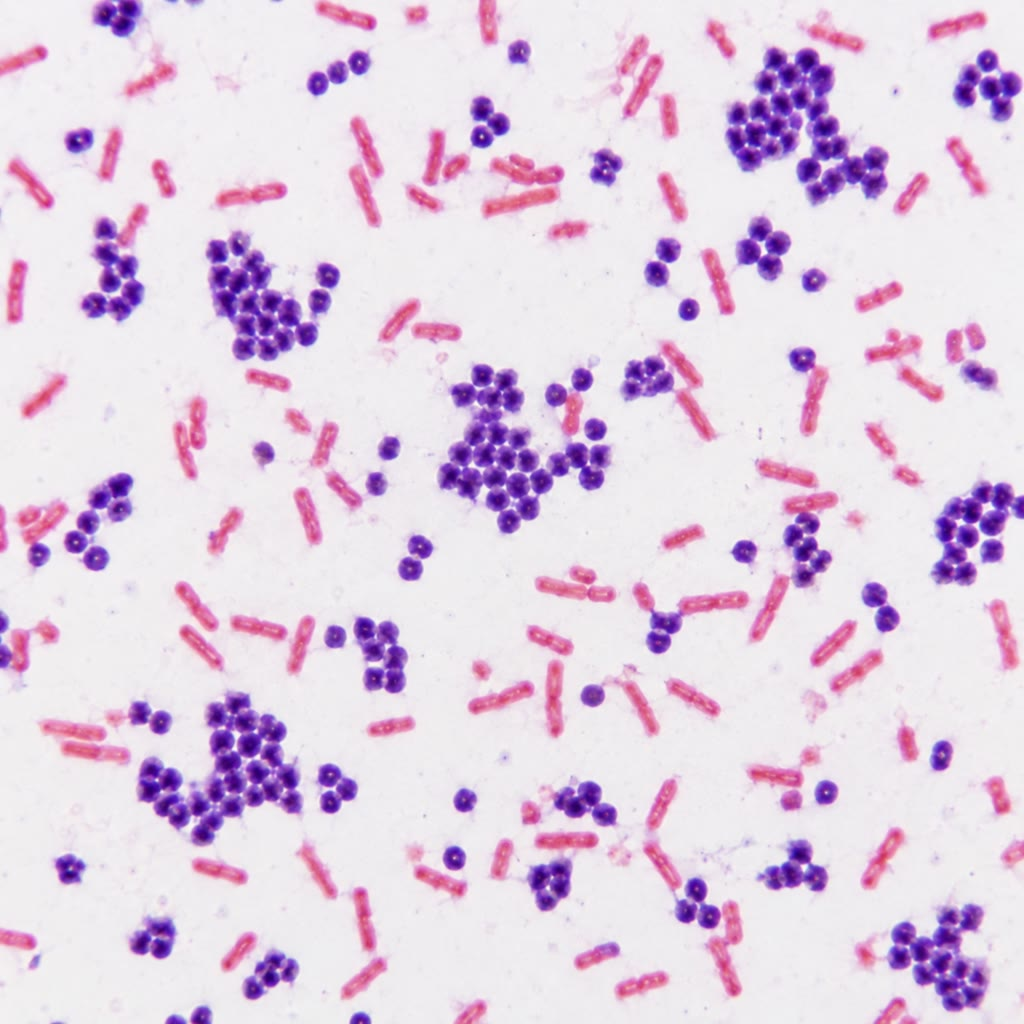
\includegraphics[width=0.36\linewidth]{images/book5/ai/b5-12-gram-stain.jpg}\hspace{0.04\linewidth}
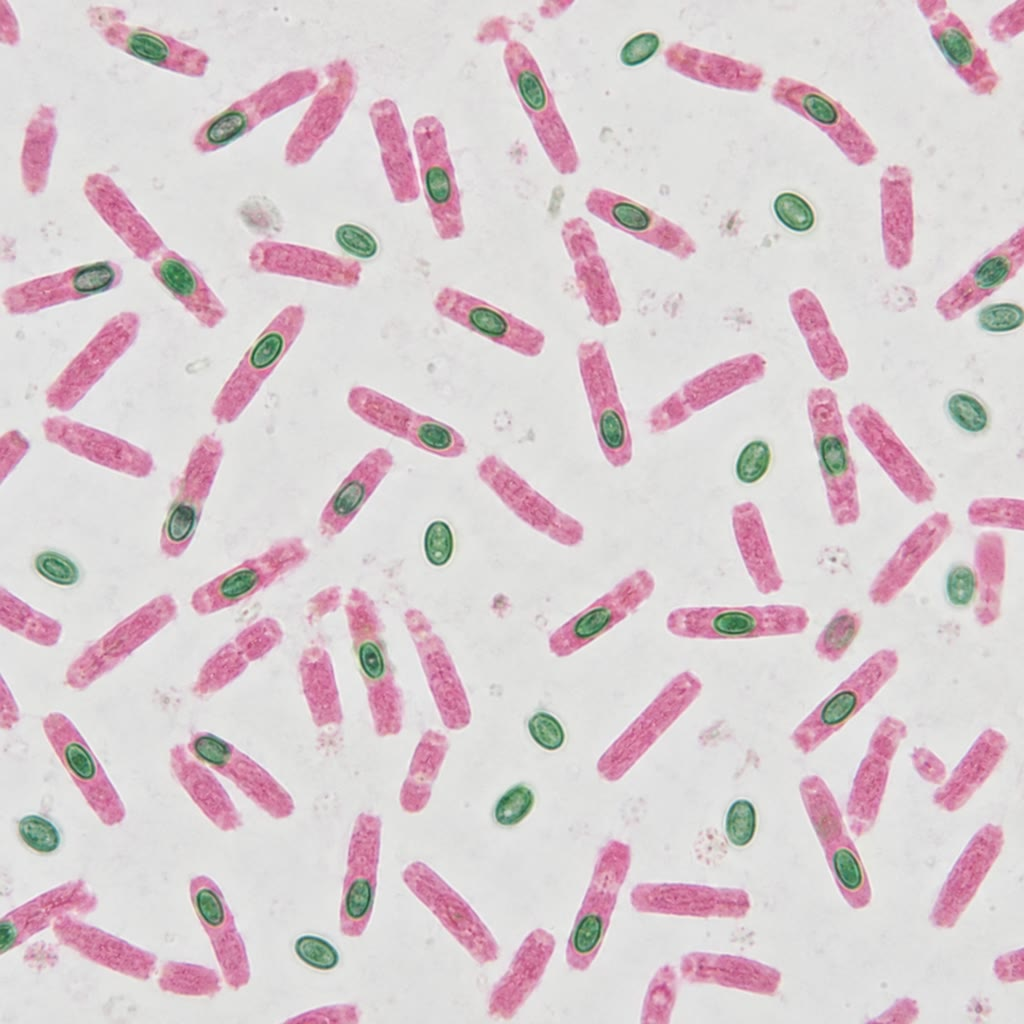
\includegraphics[width=0.36\linewidth]{images/book5/ai/b5-12-endospores.jpg}

{\small Kiri: sebuah \omterm{met:b3:bacteriology:gram}{pewarnaan Gram} --- kokus \omterm{def:b3:bacteriology:envelope}{Gram-positif} yang ungu dan
bergerombol, batang \omterm{def:b3:bacteriology:envelope}{Gram-negatif} yang merah muda. Kanan: sel \emph{Bacillus}
yang diwarnai untuk \omterm{def:b3:bacteriology:envelope}{endospora}, yakni oval hijau terang di dalam sel merah muda
dan spora bebas di sampingnya.}
\end{omfigure}

\begin{omfigure}
\begin{tikzpicture}[every node/.style={font=\scriptsize}, >=stealth]
  % Gram-positive
  \begin{scope}
    \fill[omDef!15] (0,0) rectangle (4.5,0.4); \draw[thick, omDef] (0,0) -- (4.5,0); \draw[thick, omDef] (0,0.4) -- (4.5,0.4);
    \fill[omProp!40] (0,0.5) rectangle (4.5,2.0); \foreach \y in {0.7,0.95,1.2,1.45,1.7} \draw[omProp!80!black, thin] (0,\y) -- (4.5,\y);
    \foreach \x in {0.6,1.6,2.6,3.6} \draw[omMeth!70!black, thick] (\x,0.5) -- (\x,2.3);
    \node[below] at (2.25,-0.1) {membran sitoplasma};
    \node[right, align=left] at (4.6,1.25) {peptidoglikan tebal\\(\qtyrange{20}{80}{nm})}; \node[right, omMeth!70!black] at (4.6,2.2) {asam teikoat};
    \node[above, font=\small\bfseries] at (2.25,2.5) {Gram-positif};
  \end{scope}
  % Gram-negative
  \begin{scope}[xshift=8.6cm]
    \fill[omDef!15] (0,0) rectangle (4.5,0.4); \draw[thick, omDef] (0,0) -- (4.5,0); \draw[thick, omDef] (0,0.4) -- (4.5,0.4);
    \fill[omProp!40] (0,0.75) rectangle (4.5,1.05); \draw[omProp!80!black, thin] (0,0.9) -- (4.5,0.9);
    \fill[omDef!15] (0,1.5) rectangle (4.5,1.9); \draw[thick, omDef] (0,1.5) -- (4.5,1.5); \draw[thick, omDef] (0,1.9) -- (4.5,1.9);
    \foreach \x in {0.4,0.9,1.4,1.9,2.4,2.9,3.4,3.9} \draw[omThm, thick] (\x,1.9) -- (\x,2.35);
    \draw[thick, fill=white] (2.0,1.45) rectangle (2.5,1.95); \node[below, font=\tiny] at (2.25,1.45) {porin};
    \node[below] at (2.25,-0.1) {membran sitoplasma};
    \node[right] at (4.6,0.9) {peptidoglikan tipis}; \node[right] at (4.6,1.7) {membran luar}; \node[right, omThm] at (4.6,2.25) {LPS (endotoksin)};
    \node[right, font=\tiny] at (4.6,1.27) {periplasma};
    \node[above, font=\small\bfseries] at (2.25,2.5) {Gram-negatif};
  \end{scope}
\end{tikzpicture}

{\small Kedua selubungnya. \omterm{def:b3:bacteriology:envelope}{Gram-positif} membungkus membrannya dengan banyak
lapis \omterm{def:b3:bacteriology:envelope}{peptidoglikan}; \omterm{def:b3:bacteriology:envelope}{Gram-negatif} berlapis tipis dan bermembran luar dari
\omterm{def:b3:bacteriology:envelope}{lipopolisakarida} yang ditembusi porin, yang menahan banyak
\omterm{def:b3:bacteriology:antibiotics}{antibiotik} di luar lalu membuat endotoksin yang menyebabkan renjatan septik.}
\end{omfigure}

\section{Pertumbuhan}

\begin{theorem}[Pertumbuhan eksponensial, hukum Monod, dan kemostat]\label{thm:b3:bacteriology:monod}
\index{pertumbuhan eksponensial!bakteri}\index{persamaan Monod}%
\index{kemostat}\index{laju pengenceran}
Sebuah populasi berisi $N$ sel yang membelah dengan waktu generasi $T$ tumbuh
sebagai $N(t) = N_{0}\,2^{t/T} = N_{0}e^{\mu t}$ dengan laju pertumbuhan jenis $\mu =
\ln 2/T$. Lajunya bergantung pada hara pembatas $S$ lewat
\emph{hukum Monod}
\[
\mu(S) = \mu_{\max}\,\frac{S}{K_{S} + S},
\]
yang menjenuh pada $\mu_{\max}$ dan separuh maksimum pada $S = K_{S}$. Di
dalam sebuah \emph{kemostat} --- sebuah bejana bervolume $V$ yang ke dalamnya
medium segar berkepekatan hara $S_{0}$ mengalir dengan laju $F$, dan dari
dalamnya biakannya keluar dengan laju yang sama, dengan \omterm{thm:b3:bacteriology:monod}{laju pengenceran}
$D = F/V$ --- keadaan tunaknya memenuhi
\[
\mu(S^{*}) = D,\qquad S^{*} = \frac{K_{S}D}{\mu_{\max} - D},\qquad
X^{*} = Y\,(S_{0} - S^{*}),
\]
dengan $X$ kerapatan selnya dan $Y$ perolehannya (sel yang dibuat tiap satuan
haranya). Penelitinya menetapkan laju pertumbuhannya dengan memutar sebuah
pompa; biakannya menanggapi dengan menyesuaikan hara yang ditinggalkannya. Bila
$D$ melampaui $\mu(S_{0})$ selnya tak dapat mengimbangi lalu tersapu keluar.
\end{theorem}
\begin{proof}
Selnya: $\mathrm{d}X/\mathrm{d}t = \mu(S)X - DX$, yakni pertumbuhan dikurangi
aliran keluar; pada keadaan tunak dengan $X^{*} > 0$, $\mu(S^{*}) = D$, dan
membalikkan hukum Monodnya memberi $S^{*}$. Haranya: $\mathrm{d}S/\mathrm{d}t = D(S_{0} -
S) - \mu(S)X/Y$, yakni aliran masuk dikurangi aliran keluar dikurangi
pemakaiannya; pada keadaan tunak, dengan $\mu = D$, $D(S_{0} - S^{*}) = DX^{*}/Y$,
sehingga diperoleh $X^{*}$. Keadaan tunaknya ada hanya bila $S^{*} < S_{0}$,
yakni $D <
\mu(S_{0})$; di seberangnya satu-satunya keadaan tunaknya adalah $X = 0$, yakni
tersapu keluar. Kemantapannya: bila $X$ naik di atas $X^{*}$ ia memakai lebih
banyak, $S$ turun di bawah $S^{*}$, $\mu$ turun di bawah $D$, lalu $X$ menurun
--- yakni sebuah umpan balik negatif lewat haranya.
\end{proof}

\begin{example}[Sebuah biakan dalam angka]\label{ex:b3:bacteriology:numbers}
\emph{E.~coli} di dalam medium kaya pada \qty{37}{\celsius}: $T = \qty{20}{min}$,
$\mu = \qty{2.1}{h^{-1}}$. Dari satu sel, jumlahnya $2^{36}$ sesudah dua belas
jam --- yakni $7\times 10^{10}$ sel, kira-kira \qty{70}{mg}, dan di situlah
sebuah labu \qty{100}{mL} berhenti karena kekurangan oksigen dan gula; ``bobot
Bumi dalam dua hari'' itu $2^{144}\approx 10^{43}$ sel, dan aritmetikanya hanya
menunjukkan bahwa pertumbuhan eksponensial tak pernah bertahan lama. Di dalam
sebuah kemostat pada glukosa dengan $\mu_{\max} = \qty{1.0}{h^{-1}}$, $K_{S} =
\qty{0.01}{g/L}$, $S_{0} = \qty{1}{g/L}$, dan $Y = \qty{0.5}{g}$ sel
tiap gram glukosa, \omterm{thm:b3:bacteriology:monod}{laju pengenceran} \qty{0.5}{h^{-1}} menyisakan $S^{*}
= 0.01\times 0.5/0.5 = \qty{0.01}{g/L}$ glukosa lalu menahan $X^{*} =
\qty{0.495}{g/L}$ sel, yang membelah tiap \qty{83}{min}, tanpa batas.
Kemostat adalah cara fisiologi pada laju pertumbuhan yang tetap dikaji, dan
cara ribuan generasi evolusi dijalankan di dalam sebuah botol.
\end{example}

\begin{omfigure}
\begin{tikzpicture}
\begin{axis}[
  width=6.6cm, height=5.4cm,
  axis x line=bottom, axis y line=left,
  xmin=0, xmax=14, ymin=1e6, ymax=1e10, ymode=log,
  xlabel={jam}, ylabel={sel tiap mL},
  xlabel style={font=\small, at={(axis description cs:0.5,-0.12)}, anchor=north}, ylabel style={font=\small},
  tick label style={font=\scriptsize}, xtick={0,4,8,12},
  clip=false,
]
\addplot[very thick, omDef, domain=0:1.5, samples=2] {1e6};
\addplot[very thick, omDef, domain=1.5:7.5, samples=40] {1e6*2^((x-1.5)/0.5)};
\addplot[very thick, omDef, domain=7.5:12, samples=2] {4.1e9};
\addplot[very thick, omDef, domain=12:14, samples=10] {4.1e9*exp(-0.15*(x-12))};
\node[font=\scriptsize, anchor=south] at (axis cs:0.8,1.2e6) {senjang};
\node[font=\scriptsize, anchor=west] at (axis cs:2.5,3e8) {eksponensial: $T = \qty{30}{min}$};
\node[font=\scriptsize, anchor=north] at (axis cs:10,3.5e9) {stasioner};
\node[font=\scriptsize, anchor=north] at (axis cs:12.8,2.2e9) {kematian};
\end{axis}
\begin{axis}[
  at={(7.8cm,0)}, anchor=south west,
  width=6.6cm, height=5.4cm,
  axis x line=bottom, axis y line=left,
  xmin=0, xmax=0.1, ymin=0, ymax=1.1,
  xlabel={glukosa $S$ (g/L)}, ylabel={$\mu$ (h$^{-1}$)},
  xlabel style={font=\small, at={(axis description cs:0.5,-0.12)}, anchor=north}, ylabel style={font=\small},
  tick label style={font=\scriptsize}, xtick={0,0.01,0.05,0.1}, xticklabels={0,$K_S$,0.05,0.1}, ytick={0,0.5,1},
  clip=false,
]
\addplot[very thick, omThm, domain=0:0.1, samples=60] {x/(0.01+x)};
\addplot[dashed, gray, domain=0:0.1, samples=2] {1};
\addplot[dashed, gray] coordinates {(0.01,0) (0.01,0.5)}; \addplot[dashed, gray] coordinates {(0,0.5) (0.01,0.5)};
\node[font=\scriptsize, omThm, anchor=north west] at (axis cs:0.045,0.6) {Monod: $\mu = \mu_{\max}S/(K_{S}+S)$};
\node[font=\scriptsize, gray, anchor=south east] at (axis cs:0.1,1.01) {$\mu_{\max}$};
\end{axis}
\end{tikzpicture}

{\small Kiri: sebuah biakan gelombang --- masa senjang selagi enzimnya
diimbas, pertumbuhan eksponensial, sebuah \omterm{def:b3:bacteriology:phases}{fase stasioner} ketika haranya habis,
dan kematian yang lambat. Kanan: hukum Monod, yakni laju pertumbuhan terhadap
hara pembatasnya, dengan $K_{S}$ kepekatan bagi pertumbuhan separuh maksimum.}
\end{omfigure}

\begin{definition}[Fase dan keadaan]\label{def:b3:bacteriology:phases}
\index{fase senjang}\index{fase stasioner}\index{sporulasi}\index{faktor sigma}
Di dalam labu yang segar (sebuah \emph{biakan gelombang}) selnya mula-mula
berhenti sejenak --- yakni \emph{fase senjang}, selagi ia mengimbas enzim yang
dituntut medium barunya --- lalu tumbuh secara eksponensial, lalu berhenti
ketika sebuah hara terkuras atau sebuah limbah menumpuk: yakni \emph{fase
stasioner}, yang di dalamnya selnya mengerut, menebalkan selubungnya,
memadatkan nukleoidnya di sekeliling protein pelindung, menyalakan gen
cekaman lewat faktor sigma alternatif RpoS, lalu dapat bertahan berbulan-bulan;
sesudahnya menyusul fase kematian yang di dalamnya sebagian besar selnya
melisis dan segelintir hidup dari sisanya. Sebagian spesies menjawab
kelaparannya dengan sebuah program perkembangan: \emph{Bacillus
subtilis} membelah secara tak setangkup lalu sel yang lebih besar menelan yang
lebih kecil kemudian membangun sporanya di sekelilingnya, yakni sebuah runtunan
delapan jam yang dikendalikan riam \emph{faktor sigma} --- yakni subunit yang
mengarahkan RNA polimerase ke satu perangkat promotor --- yang berselang-seling
antara kedua kompartemennya, yakni contoh bakteri yang pertama bagi
diferensiasi dan bagi pengisyaratan antarsel melewati sebuah dinding.
\end{definition}

\section{Saling mengindera}

\begin{definition}[Penginderaan kuorum]\label{def:b3:bacteriology:quorum}
\index{penginderaan kuorum}\index{autopengimbas}\index{sistem dua komponen}
Bakteri mendeteksi kerapatannya sendiri lewat \emph{penginderaan kuorum}: tiap
selnya menyekresikan sebuah molekul isyarat yang kecil, yakni sebuah
\emph{autopengimbas} --- lakton homoserina terasilasi pada \omterm{def:b3:bacteriology:envelope}{Gram-negatif},
peptida pendek pada \omterm{def:b3:bacteriology:envelope}{Gram-positif} --- dengan laju yang tetap; kepekatannya di
dalam mediumnya naik seiring cacah selnya, dan ketika kepekatannya melewati
sebuah ambang, molekul itu mengikat sebuah reseptor yang menyalakan seperangkat
gen, dan di antaranya sintase autopengimbasnya sendiri (dari situlah namanya).
Gen yang dikendalikannya adalah gen yang hanya berbuah dalam kebersamaan:
cahaya pada \emph{Vibrio fischeri}, faktor virulensi pada
\emph{Staphylococcus aureus} dan \emph{Pseudomonas aeruginosa}, matriks
biofilm, kompetensi bagi penyerapan DNA, serta pembunuhan tetangganya. Sebagian
besar penginderaan bakteri berjalan lewat \emph{sistem dua komponen}: sebuah
kinase histidina membran yang mendeteksi sebuah rangsangan lalu memfosforilasi
sebuah pengatur tanggapan sitoplasma, yang mengikat DNA --- dan sebuah sel
memiliki selusin lebih, bagi fosfat, osmolaritas, oksigen, serta autopengimbas
spesies lain.
\end{definition}

\begin{proof}[Bukti eksperimental]
Nealson, Platt, dan Hastings (1970) menumbuhkan bakteri laut yang bercahaya
yaitu \emph{Vibrio fischeri} dari inokulum yang encer lalu mendapati bahwa
selnya tidak membuat cahaya sampai mencapai kerapatan sekitar $10^{7}$ tiap
mililiter, lalu semuanya menyala bersama; medium yang di dalamnya sebuah biakan
pekat telah tumbuh, bila disterilkan lalu ditambahkan pada biakan yang encer,
menyalakan cahayanya seketika. Selnya menghitung sebuah zat yang disekresikan,
bukan menghitung waktu atau haranya. Zat itu dikenali sebagai sebuah lakton
asil-homoserina (Eberhard, 1981), dan gennya --- \emph{luxI} bagi sintasenya,
\emph{luxR} bagi reseptornya, serta operon lusiferase yang dikendalikannya ---
diklon ke dalam \emph{E.~coli}, yang lalu bersinar ketika berjejal. Di dalam
cumi-cumi yang memelihara bakterinya pada $10^{10}$ tiap mililiter, organ
cahayanya bersinar; di laut, tempat bakterinya encer, bakterinya gelap lalu
menghemat ongkosnya.
\end{proof}

\begin{proposition}[Sebuah ambang kerapatan]\label{prop:b3:bacteriology:threshold}
\index{penginderaan kuorum!ambang}
Misalkan tiap dari $N$ sel di dalam volume $V$ menyekresikan \omterm{def:b3:bacteriology:quorum}{autopengimbas}
dengan laju $p$ molekul tiap detik, dan misalkan molekulnya hilang (terurai
atau terencerkan) dengan laju orde satu $k$. Kepekatannya mendekati
$A^{*} = pN/(kV)$, sebanding dengan kerapatan sel $N/V$, dengan
tetapan waktu $1/k$; reseptornya menyala ketika $A^{*}$ mencapai
ambangnya $A_{\text{amb}}$, yakni pada kerapatan
\[
\left(\frac{N}{V}\right)_{\text{amb}} = \frac{k\,A_{\text{amb}}}{p}.
\]
Di dalam ruang tertutup --- organ cahaya seekor cumi-cumi, sebuah abses, lendir
sebuah paru-paru --- $k$ kecil karena isyaratnya tidak terbawa pergi, sehingga
kerapatan ambangnya tercapai oleh lebih sedikit sel; di perairan terbuka
ambangnya tak pernah tercapai. Karena itu selnya mengukur bukan cacahnya
melainkan cacahnya tiap satuan volume yang dibaginya, dan itulah yang berarti
bagi tindakan bekerja sama apa pun, dan umpan balik positif \omterm{def:b3:bacteriology:quorum}{autopengimbasnya}
pada sintasenya sendiri membuat sakelarnya tajam: begitu beberapa sel melewati
ambangnya, keluaran tambahannya mendorong sisanya ikut melewatinya.
\end{proposition}
\begin{proof}
$\mathrm{d}A/\mathrm{d}t = pN/V - kA$ memiliki keadaan tunak $A^{*} =
pN/(kV)$ lalu melemas menujunya sebagai $e^{-kt}$. Menetapkan $A^{*} = A_{\text{amb}}$
lalu menyelesaikannya bagi $N/V$ memberi kerapatan ambangnya.
\end{proof}

\begin{omfigure}
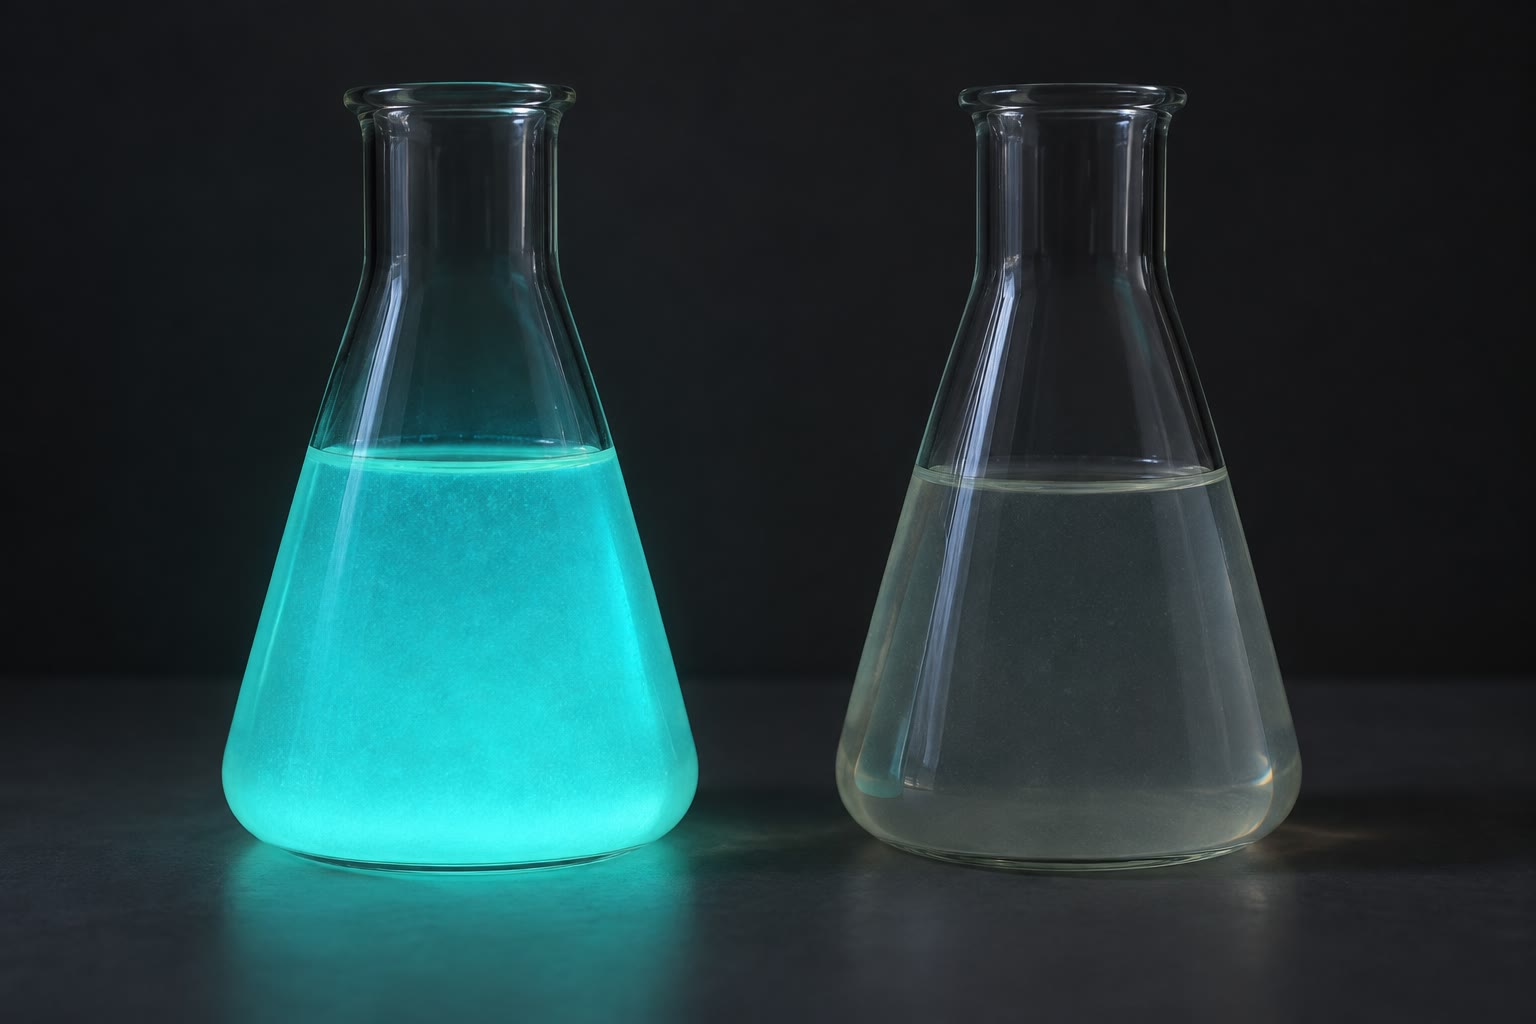
\includegraphics[width=0.46\linewidth]{images/book5/ai/b5-12-quorum-glow.jpg}\hspace{0.04\linewidth}
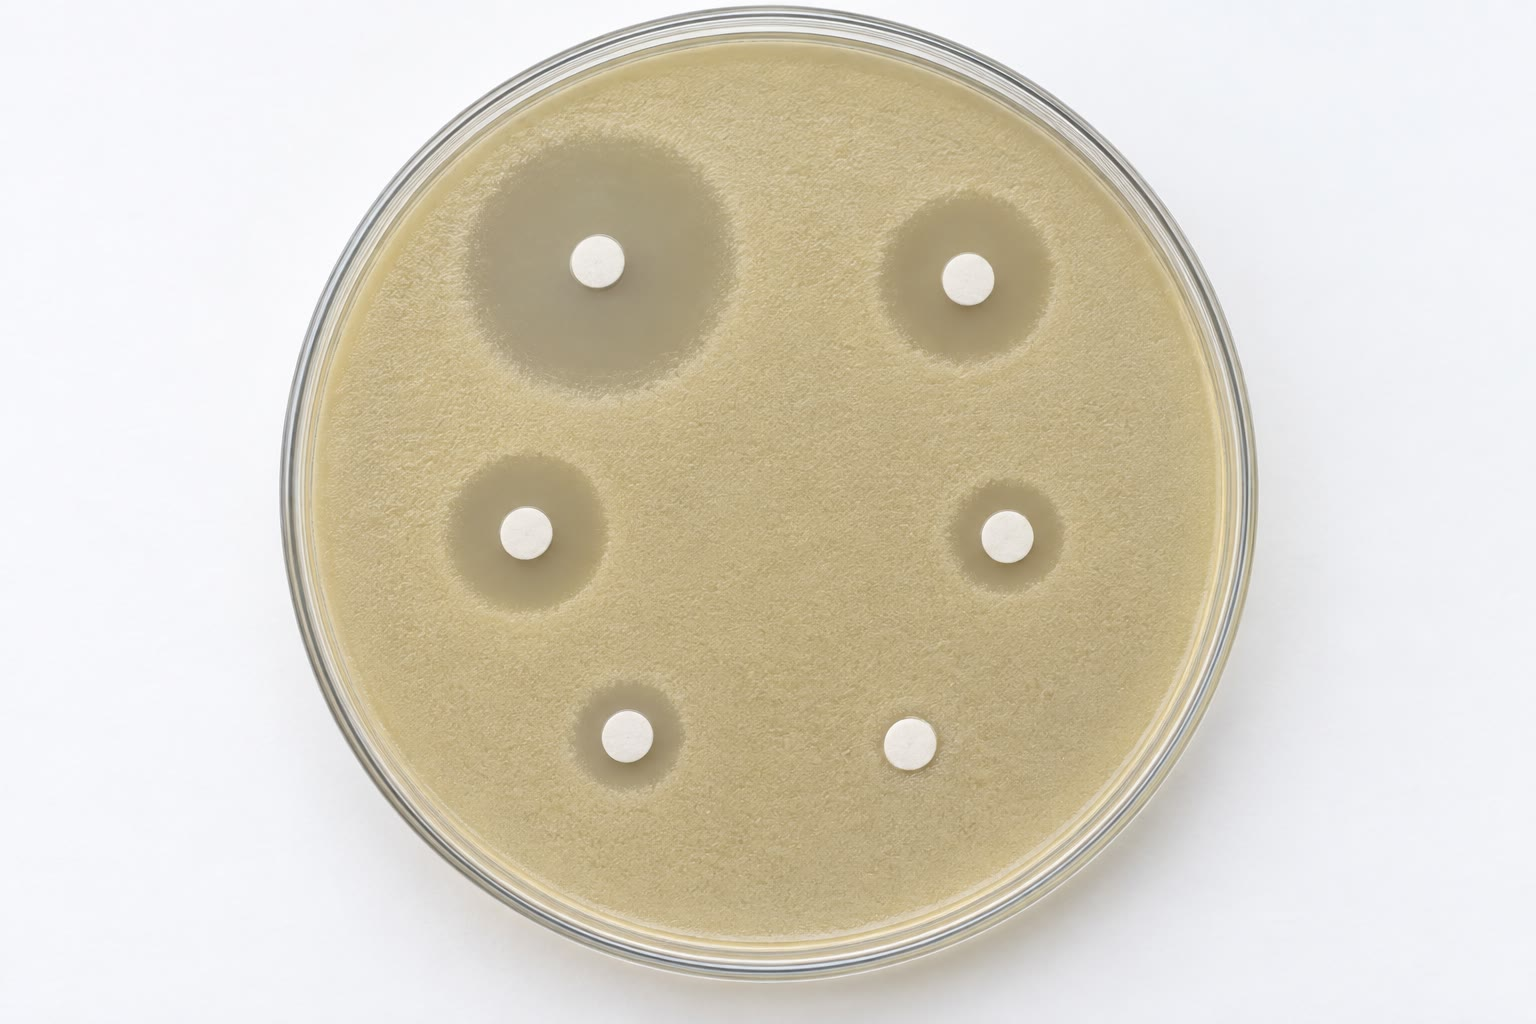
\includegraphics[width=0.46\linewidth]{images/book5/ai/b5-12-antibiotic-disks.jpg}

{\small Kiri: sebuah biakan pekat \emph{Vibrio fischeri} yang bersinar, di
samping biakan encer yang gelap --- yakni sel yang sama, di atas dan di bawah
kuorumnya. Kanan: sebuah uji \omterm{met:b3:bacteriology:mic}{difusi cakram}; garis tengah tiap zona beningnya
mengukur kepekaan bakterinya terhadap \omterm{def:b3:bacteriology:antibiotics}{antibiotik} pada cakram itu,
dan cakram yang tak berzona menandai sebuah kekebalan.}
\end{omfigure}

\section{Lalu lintas gen}

\begin{definition}[Pemindahan gen mendatar]\label{def:b3:bacteriology:hgt}
\index{transformasi}\index{transduksi}\index{konjugasi}%
\index{plasmid!kekebalan}\index{unsur genetik bergerak}\index{pangenom}
Bakteri berbiak secara klonal tetapi mempertukarkan gen lewat tiga rute.
\emph{Transformasi}: penyerapan DNA telanjang dari lingkungannya oleh sebuah
sel yang kompeten --- yakni rute yang lewatnya pneumokokus Griffith memperoleh
kapsulnya dan Avery menunjukkan bahwa asas pentransformasinya adalah DNA
(1944). \emph{Transduksi}: sebuah fag yang mengemas sepotong DNA inangnya lalu
menyuntikkannya ke inang berikutnya (\cref{ch:b3:virology}).
\emph{Konjugasi}: pemindahan sebuah \omterm{def:b3:genetic-engineering:tools}{plasmid} lewat sebuah pilus dan sebuah
jembatan kawin dari pendonor yang membawanya ke penerimanya, yang diperagakan
Lederberg dan Tatum (1946) dengan galur auksotrof \emph{E.~coli}
yang menghasilkan rekombinan prototrof hanya ketika dicampurkan. \omterm{def:b3:genetic-engineering:tools}{Plasmid}
konjugatif mengusung gen pemindahnya sendiri; banyak di antaranya juga
mengusung gen kekebalan, yang kerap mengelompok di dalam \emph{integron} dan
diapit transposon, sehingga satu perkawinan dapat memindahkan kekebalan
terhadap lima \omterm{def:b3:bacteriology:antibiotics}{antibiotik} sekaligus, melintasi spesies. Akibatnya sebuah spesies
bakteri memiliki genom inti yang dimiliki semua galurnya dan genom tambahan
yang beragam --- yakni sebuah \emph{pangenom}: dua galur \emph{E.~coli} boleh
jadi berbeda seperlima gennya, dan galur patogennya berbeda dari yang tak
berbahaya terutama lewat pulau gen virulensi yang diperolehnya. Gen bab mutasi
jilid Tahun~2 timbul lewat mutasi; gen bab ini sebagian besar berdatangan.
\end{definition}

\begin{omfigure}
\begin{tikzpicture}[every node/.style={font=\scriptsize}, >=stealth]
  % transformation
  \begin{scope}
    \draw[thick, fill=omDef!15] (0,0) ellipse (1.0 and 0.55);
    \draw[omThm, very thick] (-1.9,0.6) .. controls (-1.5,0.8) .. (-1.2,0.5); \draw[->, omThm, thick] (-1.2,0.5) -- (-0.7,0.25);
    \node[below, align=center] at (0,-0.7) {transformasi:\\DNA telanjang diserap\\sel yang kompeten};
  \end{scope}
  % transduction
  \begin{scope}[xshift=4.6cm]
    \draw[thick, fill=omDef!15] (0,0) ellipse (1.0 and 0.55);
    \draw[thick, fill=omProp!40] (-1.3,1.0) -- (-1.0,1.3) -- (-0.7,1.0) -- (-1.0,0.7) -- cycle; \draw[thick] (-1.0,0.7) -- (-0.9,0.35);
    \draw[omThm, very thick] (-1.1,1.15) -- (-0.9,0.85);
    \node[below, align=center] at (0,-0.7) {transduksi:\\sebuah fag mengusung sepotong\\DNA inang terakhirnya};
  \end{scope}
  % conjugation
  \begin{scope}[xshift=9.6cm]
    \draw[thick, fill=omDef!15] (-1.3,0) ellipse (0.9 and 0.5); \draw[thick, fill=omDef!15] (1.3,0) ellipse (0.9 and 0.5);
    \draw[very thick, omMeth!70!black] (-0.4,0) -- (0.4,0);
    \draw[omThm, very thick] (-1.5,0) circle (0.25); \draw[->, omThm, thick] (-1.25,0) -- (1.0,0);
    \node[below, align=center] at (0,-0.7) {konjugasi:\\sebuah plasmid menyeberangi\\jembatan kawin};
  \end{scope}
\end{tikzpicture}

{\small Ketiga rute pemindahan mendatarnya. Gen bagi kekebalan,
virulensi, dan metabolisme berpindah antarsel --- dan antarspesies ---
lebih cepat daripada yang dapat dibuat mutasi.}
\end{omfigure}

\begin{proof}[Bukti eksperimental]
Robert Koch (1876--1884) menegakkan bahwa sebuah bakteri tertentu menyebabkan
penyakit tertentu: ia memisahkan \emph{Bacillus anthracis} dari hewan yang
sakit, menumbuhkannya sebagai biakan murni pada medium padat (pelat agar dan
koloni tunggal adalah temuan laboratoriumnya), menunjukkan bahwa biakannya
menghasilkan ulang antraks pada hewan yang sehat dan dapat dipisahkan kembali
darinya --- yakni postulat yang sampai kini menetapkan sebuah patogen --- lalu
melanjut ke basil tuberkel dan vibrio kolera. Alexander Fleming
(1928) memperhatikan bahwa sejenis jamur yang mencemari sebuah pelat
stafilokokus telah membersihkan sebuah zona di sekelilingnya; zatnya, yakni
penisilin, dimurnikan lalu terbukti menyembuhkan infeksi oleh Florey dan Chain
(1940--1941), dan dalam sedasawarsa stafilokokus kebal yang mengusung
enzim pemusnah penisilin menjadi lazim di rumah sakit --- yakni sebuah
peringatan yang diberikan Fleming sendiri pada pidato Nobelnya.
\end{proof}

\begin{omfigure}
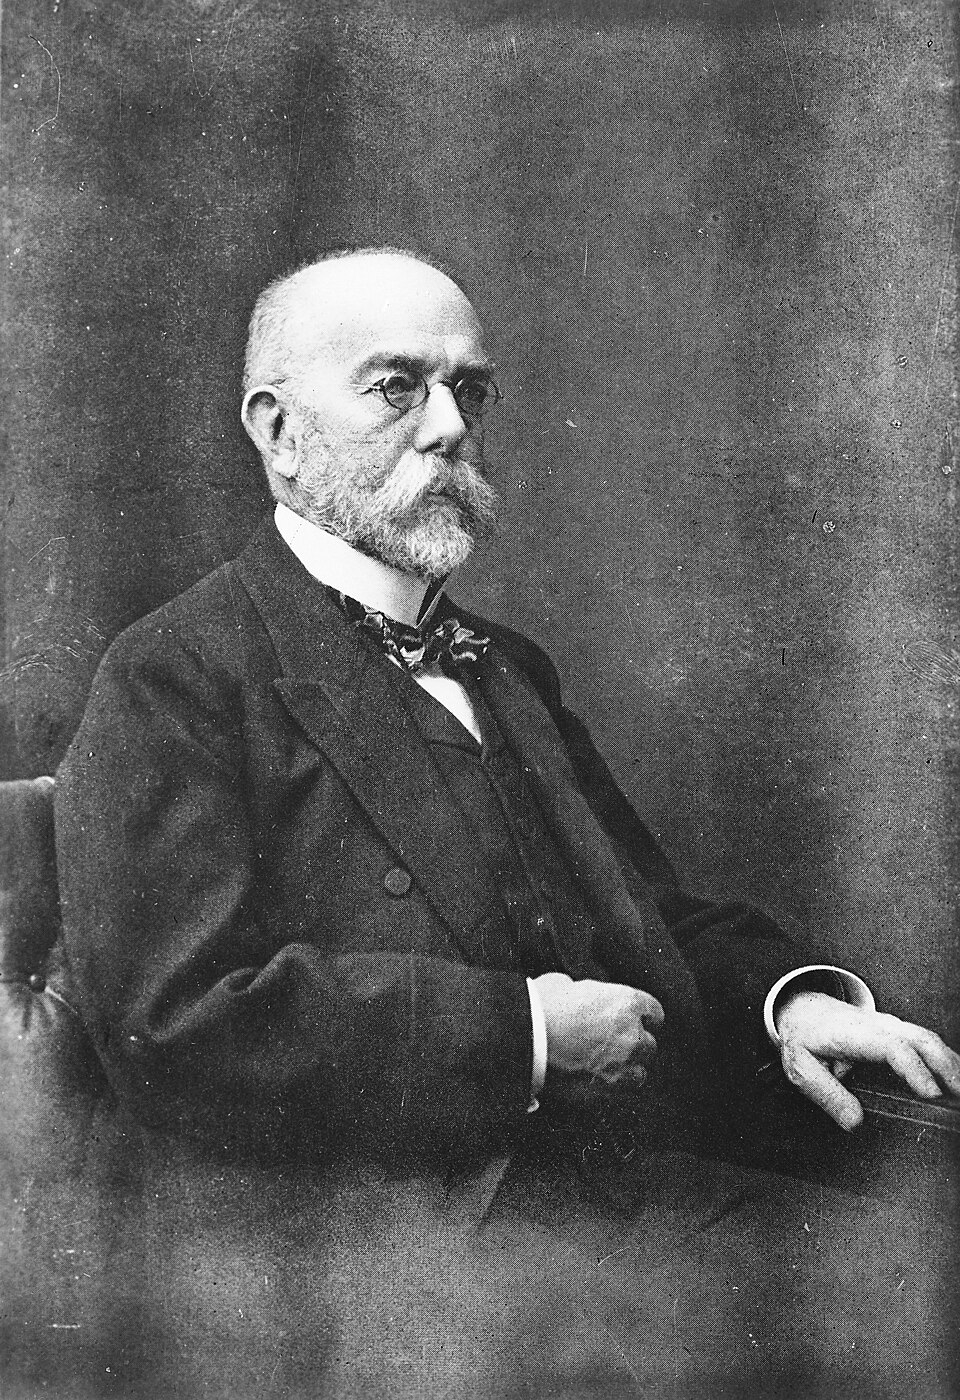
\includegraphics[width=0.30\linewidth]{images/book5/koch.jpg}\hspace{0.04\linewidth}
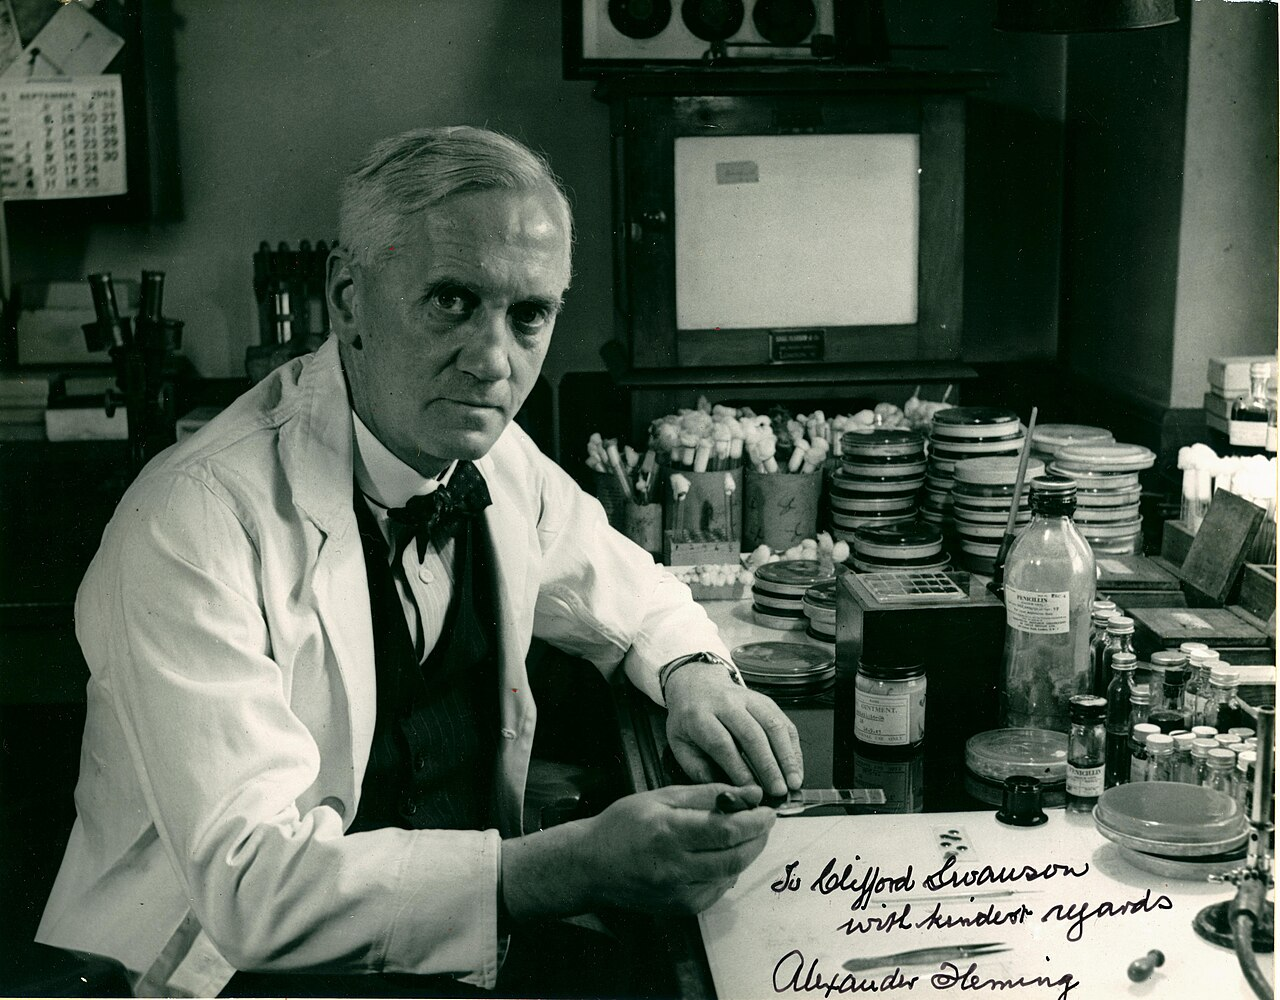
\includegraphics[width=0.56\linewidth]{images/book5/fleming.jpg}

{\small Robert Koch, yang membuktikan bahwa bakteri tertentu menyebabkan
penyakit tertentu lalu menemukan metode untuk menumbuhkannya (Wellcome
Collection, CC~BY~4.0). Kanan: Alexander Fleming di laboratoriumnya
bersama pelat jamur yang hasilnya menjadi penisilin (arsip Angkatan Laut
Amerika Serikat, domain publik).}
\end{omfigure}

\section{Antibiotik dan kekebalan}

\begin{definition}[Antibiotik]\label{def:b3:bacteriology:antibiotics}
\index{antibiotik}\index{beta-laktam}\index{ketoksikan terpilih}%
\index{kepekatan penghambat minimum}
Sebuah \emph{antibiotik} adalah molekul yang membunuh bakteri atau menghentikan
pertumbuhannya pada kepekatan yang tak berbahaya bagi inangnya, dengan bekerja
pada sasaran yang tak dimiliki inangnya atau yang dimilikinya dalam bentuk yang
berbeda --- yakni \emph{ketoksikan terpilih}. Sasarannya sedikit. Dinding
selnya: \emph{$\beta$-laktam} (penisilin, sefalosporin, karbapenem) meniru
D-Ala-D-Ala ujung peptida \omterm{def:b3:bacteriology:envelope}{peptidoglikan} lalu mengasilasi enzim yang
menaut-silangkannya, sehingga dinding yang sedang tumbuh menjadi lemah dan
selnya pecah oleh turgornya sendiri; vankomisin mengikat D-Ala-D-Ala itu
sendiri. Ribosomnya, yang bentuk bakterinya berbeda dari bentuk eukariot:
aminoglikosida (subunit kecilnya, sehingga menimbulkan salah baca), tetrasiklin
(menghalangi masuknya tRNA), makrolida dan kloramfenikol (terowongan keluar dan
peptidil transferase subunit besarnya). Girase DNA dan topoisomerase~IV:
kuinolon. RNA polimerase: rifampisin. Sintesis folat, yang tak dikerjakan
hewan: sulfonamida dan trimetoprim. Membrannya: polimiksin, yakni pilihan
terakhir. \emph{Kepekatan penghambat minimum} (MIC) adalah kepekatan obat
terendah yang mencegah pertumbuhan yang kasatmata pada sebuah galur; sebuah
galur disebut kebal ketika MIC-nya melampaui kepekatan yang dicapai obatnya di
dalam tubuh pasiennya.
\end{definition}

\begin{method}[Mengukur kepekaan]\label{met:b3:bacteriology:mic}
\index{difusi cakram}\index{pengenceran kaldu}
Ada dua uji. \emph{\omterm{met:b3:bacteriology:mic}{Pengenceran kaldu}}: inokulasikanlah sejumlah sel yang tetap
(kira-kira $5\times 10^{5}$ tiap mililiter) ke dalam sederet tabung atau sumur
yang memuat \omterm{def:b3:bacteriology:antibiotics}{antibiotiknya} dalam langkah dua kali lipat, eramkan semalam, lalu
bacalah sumur bening yang pertama: kepekatan itulah MIC-nya. \emph{\omterm{met:b3:bacteriology:mic}{Difusi
cakram}}: tebarkanlah galurnya pada sebuah pelat agar, letakkanlah cakram kertas
yang dimuati \omterm{def:b3:bacteriology:antibiotics}{antibiotik} dalam jumlah yang diketahui, lalu eramkan; obatnya
berdifusi keluar, kepekatannya turun terhadap jarak, dan pertumbuhannya
terhambat sampai jari-jari ketika kepekatannya menyamai MIC-nya, sehingga garis
tengah zona beningnya --- yang dibaca terhadap tabel terkalibrasi --- memberi
kepekaan bagi tiap cakramnya pada satu pelat. Kedua ujinya memakan sehari;
mengurutkan genomnya untuk mencari gen dan mutasi kekebalan yang telah dikenal
memakan waktu yang sama dan mulai menggantikannya.
\end{method}

\begin{definition}[Kekebalan]\label{def:b3:bacteriology:resistance}
\index{kekebalan antibiotik}\index{beta-laktamase}\index{pompa penyembur}\index{MRSA}
Sebuah bakteri kebal terhadap \omterm{def:b3:bacteriology:antibiotics}{antibiotik} lewat salah satu dari lima cara. Ia
memusnahkan obatnya: \emph{$\beta$-laktamase} menghidrolisis cincin
$\beta$-laktamnya, dan varian berspektrum luas serta karbapenemasenya kini
memusnahkan obat yang terbaru. Ia mengubah sasarannya: sebuah mutasi pada
protein ribosom atau girase yang diikat obatnya, atau, pada MRSA
(\emph{Staphylococcus aureus} yang kebal metisilin), sebuah gen yang
diperolehnya bagi enzim penaut silang yang tak diikat $\beta$-laktam;
kekebalan terhadap vankomisin mengganti D-Ala ujungnya dengan D-laktat, yang
tak dikenali obatnya. Ia memompa obatnya keluar dengan \emph{pompa penyembur},
yang kerap luas kekhasannya. Ia menghentikan masuknya obat, dengan kehilangan
sebuah porin. Atau ia memutari langkah yang terhalang dengan enzim alternatif.
Mutasi sasarannya timbul secara kebetulan di dalam tubuh pasiennya pada laju
$10^{-8}$ sampai $10^{-6}$ tiap pembelahan lalu terpilih selama pengobatannya;
enzim dan pompanya sebagian besar diperoleh pada \omterm{def:b3:genetic-engineering:tools}{plasmid} dari cadangan besar
bakteri tanah dan usus, yang di dalamnya keduanya berevolusi sepanjang zaman
melawan \omterm{def:b3:bacteriology:antibiotics}{antibiotik} yang dibuat fungi dan bakteri lain. Persister --- yakni sel
tidur yang bertahan dari sebuah obat tanpa kebal secara genetik --- menjelaskan
kekambuhan sesudah pengobatan yang semestinya berhasil.
\end{definition}

\begin{proposition}[Mengapa kekebalan tak terhindarkan dan gabungan menjadi jawabannya]\label{prop:b3:bacteriology:selection}
\index{kekebalan!seleksi}\index{terapi gabungan!antibiotik}
Sebuah infeksi berisi $10^{9}$ sel yang diobati dengan obat yang mutasi
kekebalannya timbul pada $10^{-8}$ tiap pembelahan sudah memuat
kira-kira sepuluh sel kebal; obatnya membunuh sisanya lalu kesepuluh sel itu
mengambil alih --- yakni aritmetika \cref{ch:b3:cancer-biology} persis, karena
sebuah populasi bakteri dan sebuah \omterm{def:b3:cancer-biology:hallmarks}{tumor} sama-sama klon yang berevolusi di
bawah seleksi. Dua obat dengan sasaran yang saling bebas menghadapi sebuah sel
kebal ganda pada $10^{-16}$ tiap pembelahan, yang tak dimuat semiliar sel.
Itulah sebabnya tuberkulosis, yang lesinya menahan $10^{8}$--$10^{9}$ basil,
telah diobati dengan tiga atau empat obat sekaligus sejak dasawarsa 1950-an dan
sebabnya monoterapi atasnya menghasilkan kekebalan dalam hitungan bulan; itulah
pula sebabnya setiap pemakaian \omterm{def:b3:bacteriology:antibiotics}{antibiotik}, pada seorang pasien atau di sebuah
kandang penggemukan, memilih kekebalan di suatu tempat, dan sebabnya laju
\omterm{def:b3:bacteriology:antibiotics}{antibiotik} baru --- tak satu pun dari kelas baru melawan \omterm{def:b3:bacteriology:envelope}{Gram-negatif} sejak
dasawarsa 1960-an --- menjadi ukuran yang terhadapnya kerugiannya dihitung.
Penawarnya sama dengan penawar sebuah pertandingan evolusi mana pun: pakailah
lebih sedikit, gabungkanlah, tuntaskanlah kursusnya agar sel yang sebagian
kebal tak bertahan untuk berbiak, dan carilah sasaran yang baru.
\end{proposition}

\begin{example}[Jendela seleksi mutan]\label{ex:b3:bacteriology:window}
Sebuah galur ber-MIC \qty{1}{mg/L}; mutan kebal langkah pertamanya, yang hadir
pada satu dari $10^{7}$, ber-MIC \qty{8}{mg/L}. Sebuah dosis yang menahan
obatnya pada \qty{4}{mg/L} membunuh tipe liarnya lalu membiarkan mutannya
tumbuh tanpa persaingan: rentang kepekatan antara MIC tipe liarnya dan MIC
mutannya disebut \emph{jendela seleksi mutan}, dan sebuah pengobatan yang duduk
di dalamnya membiakkan kekebalan. Sebuah dosis di atas \qty{8}{mg/L} membunuh
keduanya; dosis yang terlalu rendah, atau kursus yang dihentikan ketika
pasiennya merasa membaik dan kadar obatnya sedang turun melewati jendelanya,
itulah cara sebuah populasi yang kebal dibuat. Logika yang sama menetapkan
regimen pengobatan tuberkulosis: enam bulan, empat obat, pada dosis di atas
MIC tiap mutan langkah tunggalnya.
\end{example}

\begin{omfigure}
\begin{tikzpicture}
\begin{axis}[
  width=0.7\linewidth, height=5.6cm,
  axis x line=bottom, axis y line=left,
  xmin=0, xmax=24, ymin=0.25, ymax=32, ymode=log,
  xlabel={jam sesudah sedosis}, ylabel={obat di dalam plasma (mg/L)},
  xlabel style={font=\small, at={(axis description cs:0.5,-0.12)}, anchor=north}, ylabel style={font=\small},
  tick label style={font=\small}, xtick={0,6,12,18,24}, ytick={0.5,1,2,4,8,16}, yticklabels={0.5,1,2,4,8,16},
  clip=false,
]
\fill[omThm!15] (axis cs:0,1) rectangle (axis cs:24,8);
\addplot[very thick, omDef, domain=0:24, samples=60] {16*exp(-0.15*x)};
\addplot[dashed, gray, domain=0:24, samples=2] {1}; \addplot[dashed, gray, domain=0:24, samples=2] {8};
\node[font=\scriptsize, gray, anchor=south west] at (axis cs:0.3,1.05) {MIC tipe liarnya};
\node[font=\scriptsize, gray, anchor=south east] at (axis cs:23.7,8.4) {MIC mutan langkah pertamanya};
\node[font=\scriptsize, omThm!70!black, anchor=west] at (axis cs:13,3.5) {jendela seleksi mutan};
\node[font=\scriptsize, omDef, anchor=south west] at (axis cs:2,13) {kadar plasma sesudah sedosis};
\end{axis}
\end{tikzpicture}

{\small Jendela seleksi mutannya. Kadar obat di atas MIC mutannya membunuh
segalanya; di antara kedua MIC-nya (yang diarsir) obatnya membunuh tipe
liarnya lalu memilih mutannya. Sebuah dosis yang kadarnya jatuh melewati
jendelanya berjam-jam, atau kursus yang dihentikan dini, membiakkan kekebalan.}
\end{omfigure}

\begin{remark}[Sebagian besar bakteri bukan patogen]\label{rem:b3:bacteriology:most}
Bakteri klinik bab ini hanyalah minoritas yang sangat kecil. Dari
sejuta spesies yang ditaksir, beberapa ratus menyebabkan penyakit manusia;
sisanya menjalankan daur nitrogen, belerang, dan karbon (jilid Tahun~2),
mengikat nitrogen tiap kacang-kacangan, mencerna selulosa tiap hewan pemamah
biak, serta menyusun mikrobiom \cref{ch:b3:microbiomes}, yang hilangnya
di bawah pengobatan \omterm{def:b3:bacteriology:antibiotics}{antibiotik} menjadi ongkos tiap kursusnya. \omterm{def:b3:bacteriology:antibiotics}{Antibiotiknya}
sendiri adalah molekul mereka --- yakni senjata dan isyarat yang berevolusi di
antara bakteri tanah dan fungi jauh sebelum ada rumah sakit --- dan begitu pula
sebagian besar gen kekebalannya.
\end{remark}

\section{Latihan}

\begin{exercise}[$\star$]\label{exo:b3:bacteriology:1}
Uraikanlah selubung \omterm{def:b3:bacteriology:envelope}{Gram-positif} dan \omterm{def:b3:bacteriology:envelope}{Gram-negatif} lalu jelaskan mengapa
\omterm{met:b3:bacteriology:gram}{pewarnaan Gram} membedakan keduanya.
\end{exercise}

\begin{exercise}[$\star$]\label{exo:b3:bacteriology:2}
Sebuah biakan berisi $10^{3}$ sel tiap mililiter mencapai $10^{9}$ dalam
\qty{8}{h} pertumbuhan eksponensial. Carilah cacah generasinya, waktu
generasinya, dan $\mu$.
\end{exercise}

\begin{exercise}[$\star$]\label{exo:b3:bacteriology:3}
Sebutkanlah ketiga rute pemindahan gen mendatar lalu berikan percobaan klasik
yang memperagakan masing-masing.
\end{exercise}

\begin{exercise}[$\star$]\label{exo:b3:bacteriology:4}
Berikanlah sasaran penisilin, streptomisin, siprofloksasin, dan
rifampisin, lalu katakan mengapa masing-masing beracun secara terpilih.
\end{exercise}

\begin{exercise}[$\star\star$]\label{exo:b3:bacteriology:5}
Sebuah kemostat memiliki $\mu_{\max} = \qty{0.8}{h^{-1}}$, $K_{S} =
\qty{0.02}{g/L}$, $S_{0} = \qty{2}{g/L}$, $Y = 0.4$. Hitunglah $S^{*}$ dan
$X^{*}$ pada $D = 0.2$, $0.6$, dan $0.79$ h$^{-1}$, serta \omterm{thm:b3:bacteriology:monod}{laju pengenceran}
ketika penyapuannya mulai.
\end{exercise}

\begin{exercise}[$\star\star$]\label{exo:b3:bacteriology:6}
Dengan \cref{prop:b3:bacteriology:threshold}, bandingkanlah kerapatan ambang
bagi \omterm{def:b3:bacteriology:quorum}{penginderaan kuorum} di dalam organ cahaya cumi-cumi ($k =
\qty{0.01}{h^{-1}}$) dan di dalam air laut yang mengalir ($k = \qty{10}{h^{-1}}$),
dengan $p = 100$ molekul tiap sel tiap jam dan $A_{\text{amb}} =
\qty{10}{nmol/L}$ ($6\times 10^{12}$ molekul tiap liter).
\end{exercise}

\begin{exercise}[$\star\star$]\label{exo:b3:bacteriology:7}
Sebuah pelat \omterm{met:b3:bacteriology:mic}{difusi cakram} memperlihatkan zona $25$, $12$, dan \qty{0}{mm} bagi
tiga obat. Tafsirkanlah masing-masing, lalu jelaskan mengapa garis tengah
sebuah zona dapat diubah menjadi sebuah MIC.
\end{exercise}

\begin{exercise}[$\star\star$]\label{exo:b3:bacteriology:8}
Jelaskanlah bagaimana satu peristiwa \omterm{def:b3:bacteriology:hgt}{konjugasi} dapat membuat sebuah
\emph{Klebsiella} yang peka menjadi kebal terhadap lima \omterm{def:b3:bacteriology:antibiotics}{antibiotik}, dan mengapa
gen kekebalan begitu sering ditemukan bersama pada \omterm{def:b3:genetic-engineering:tools}{plasmid}.
\end{exercise}

\begin{exercise}[$\star\star$]\label{exo:b3:bacteriology:9}
Seorang pasien memiliki $10^{9}$ bakteri lalu memakai sebuah obat yang
kekebalannya timbul pada $10^{-7}$ tiap pembelahan. Hitunglah harapan cacah
sel kebalnya pada awalnya; lalu dengan dua obat yang saling bebas. Mengapa
persister menjadi masalah yang berbeda?
\end{exercise}

\begin{exercise}[$\star\star\star$]\label{exo:b3:bacteriology:10}
Tunjukkanlah bahwa keadaan tunak kemostatnya mantap: usiklah $X$ sedikit
di atas $X^{*}$ lalu ikuti tanda $\mathrm{d}S/\mathrm{d}t$ dan
$\mathrm{d}X/\mathrm{d}t$. Lalu jelaskanlah mengapa dua spesies yang bersaing
memperebutkan satu hara di dalam sebuah kemostat tak dapat hidup berdampingan
pada keadaan tunak, dan spesies mana yang menang pada $D$ tertentu.
\end{exercise}

\begin{exercise}[$\star\star\star$]\label{exo:b3:bacteriology:11}
\omterm{def:b3:bacteriology:quorum}{Autopengimbasnya} mengimbas sintasenya sendiri. Ubahlah model
\cref{prop:b3:bacteriology:threshold} sehingga $p$ melompat dari $p_{0}$ ke
$p_{1} \gg p_{0}$ ketika $A > A_{\text{amb}}$, lalu tunjukkan bahwa sistemnya
dapat memiliki dua keadaan mantap pada sebuah rentang kerapatan (histeresis):
sebuah populasi yang telah menyala tetap menyala pada kerapatan yang padanya
populasi yang naif akan padam. Apa kegunaan biologisnya?
\end{exercise}

\begin{exercise}[$\star\star\star$]\label{exo:b3:bacteriology:12}
Jelaskanlah jendela seleksi mutan lalu pakailah untuk mengemukakan alasan
mendukung atau menolak masing-masing hal berikut: (a) dosis tinggi bagi kursus
pendek; (b) dosis rendah bagi kursus panjang; (c) berhenti ketika gejalanya
reda; (d) \omterm{thm:b3:cancer-biology:goldie-coldman}{terapi gabungan}.
\end{exercise}

\section{Soal: Sebuah Kemostat dan Sebuah Klinik}

\begin{problem}[{Soal akhir pekan --- sebuah biakan yang ditumbuhkan di dalam
labu lalu ditahan di dalam kemostat, sebuah bakteri bercahaya yang dicacah
sampai kuorumnya, dan sebuah infeksi yang diobati melawan aritmetika
kekebalannya, berakhir pada sel di dalam kemostatnya, kerapatan ketika
cahayanya menyala, dan peluang bahwa kursus dua obat berjumpa dengan sel kebal}]
\label{pb:b3:bacteriology:1}
Data: \emph{E.~coli} pada \qty{37}{\celsius}, $T = \qty{20}{min}$; sebuah sel
berbobot \qty{1}{pg}. Kemostatnya: $V = \qty{1}{L}$, $F = \qty{0.5}{L/h}$,
$\mu_{\max} = \qty{1.0}{h^{-1}}$, $K_{S} = \qty{0.01}{g/L}$, $S_{0} =
\qty{2}{g/L}$ glukosa, $Y = 0.5$. \emph{Vibrio}: $p = 500$ molekul
\omterm{def:b3:bacteriology:quorum}{autopengimbas} tiap sel tiap jam, $A_{\text{amb}} = 6\times 10^{12}$
molekul tiap liter (\qty{10}{nmol/L}), $k = \qty{0.05}{h^{-1}}$ di dalam organ
cahayanya. Infeksinya: $10^{9}$ sel; kekebalan terhadap obat A pada
$10^{-8}$ tiap pembelahan, terhadap obat B pada $10^{-7}$; MIC tipe liar A
\qty{1}{mg/L}, mutan langkah pertamanya \qty{8}{mg/L}; sedosis memberi
\qty{16}{mg/L} yang turun dengan waktu paruh \qty{4}{h}.

\medskip
\noindent\textbf{Bagian I --- Labunya.}
\begin{enumerate}
  \item Satu sel di dalam \qty{100}{mL} kaldu. Berapa sel sesudah
        \qty{6}{h} pertumbuhan eksponensial, dan berapa kerapatannya tiap mL?
  \item Kaldunya menopang paling banyak $2\times 10^{9}$ sel tiap mL. Kapan
        pertumbuhannya berhenti, dan berapa massa sel biakannya?
  \item Berapa lama keturunan satu sel mencapai
        bobot Bumi ($6\times 10^{27}$ g)? Berikanlah komentar.
  \item \omterm{def:b3:bacteriology:phases}{Fase senjangnya} berlangsung \qty{1}{h} ketika sel dari \omterm{def:b3:bacteriology:phases}{fase stasioner}
        diinokulasikan ke dalam medium yang segar, dan nyaris tak ada ketika
        sel eksponensial yang dipakai. Jelaskanlah.
  \item Hitunglah $\mu$ dari $T$. Bila mediumnya dialihkan ke sebuah gula yang
        padanya $T = \qty{60}{min}$, berapa $\mu$-nya, dan dengan faktor
        berapa cacah selnya sesudah \qty{6}{h} turun?
  \item Sebuah contoh biakan stasionernya ditebarkan pada sebuah pelat lalu
        memberi $200$ koloni dari \qty{0.1}{mL} pengenceran $10^{-6}$.
        Berapa cacah yang hidup, dan mengapa cacah itu boleh jadi berbeda dari
        cacah di bawah mikroskop?
\end{enumerate}

\medskip
\noindent\textbf{Bagian II --- Kemostatnya.}
\begin{enumerate}[resume]
  \item Hitunglah \omterm{thm:b3:bacteriology:monod}{laju pengenceran} $D$ dan waktu generasi yang terpaksa
        diambil biakannya.
  \item Hitunglah $S^{*}$ dan $X^{*}$ (dalam g/L dan sel tiap mL).
  \item Berapa sel yang meninggalkan bejananya tiap jam? Berapa generasi
        yang dilalui biakannya dalam sebulan?
  \item Pompanya dinaikkan menjadi $F = \qty{0.95}{L/h}$. Berapa $S^{*}$ dan
        $X^{*}$ yang baru? Apa yang terjadi pada $F = \qty{1.1}{L/h}$?
  \item Sebuah mutan muncul dengan $\mu_{\max} = \qty{1.2}{h^{-1}}$ dan
        $K_{S}$ yang sama. Pada $D = 0.5$, berapa $S^{*}$ yang dituntutnya, dan
        apa yang terjadi pada galur aslinya? (Pakailah
        \cref{exo:b3:bacteriology:10}.)
  \item Sebulan berjalan berarti $700$ generasi. Bila sebuah mutasi yang
        menguntungkan timbul pada $10^{-9}$ tiap pembelahan dan bejananya
        memuat $10^{12}$ sel, berapa mutasi menguntungkan yang timbul tiap
        generasi? Apa yang dikatakan hal itu tentang evolusi di dalam kemostat?
\end{enumerate}

\medskip
\noindent\textbf{Bagian III --- Kuorumnya.}
\begin{enumerate}[resume]
  \item Hitunglah kerapatan sel ambang bagi cahaya di dalam organ
        cahayanya, dalam sel tiap mL.
  \item Organ cahayanya memuat \qty{1}{\micro L} bakteri pada $10^{10}$
        tiap mL. Dengan faktor berapa \omterm{def:b3:bacteriology:quorum}{autopengimbasnya} berada di atas ambangnya?
  \item Di air laut isyaratnya tersapu pergi dengan $k = \qty{20}{h^{-1}}$.
        Berapa kerapatan ambangnya? Bandingkanlah dengan $10^{2}$ sel tiap mL
        di laut lepas.
  \item Sesudah cumi-cuminya mengeluarkan \qty{90}{\%} bakterinya saat fajar,
        berapa lama sampai sisanya yang $10^{9}$ tiap mL, yang membelah tiap
        \qty{2}{h}, memulihkan $10^{10}$ tiap mL? Apakah cahayanya padam
        sementara itu?
  \item Tiap sel yang bersinar membelanjakan kira-kira \qty{20}{\%} energinya
        bagi cahaya. Mengapa sel yang gelap dipihak di laut, dan mengapa tidak
        di dalam organnya?
  \item Sebuah patogen memakai sistem yang sama untuk menunda toksinnya sampai
        ia banyak. Usulkanlah sebuah siasat obat yang memanfaatkan hal itu lalu
        katakan mengapa siasat itu mungkin memilih kekebalan lebih lambat
        daripada sebuah \omterm{def:b3:bacteriology:antibiotics}{antibiotik}.
\end{enumerate}

\medskip
\noindent\textbf{Bagian IV --- Kliniknya.}
\begin{enumerate}[resume]
  \item Berapa harapan cacah sel yang kebal terhadap A pada awal
        pengobatannya; terhadap B; terhadap keduanya.
  \item Berapa peluang bahwa tak ada sel yang kebal terhadap A; terhadap keduanya.
  \item Sesudah sedosis, kapan kadar obatnya turun ke \qty{8}{mg/L},
        dan ke \qty{1}{mg/L}? Berapa lama tiap dosisnya berada di dalam
        jendela seleksi mutannya?
  \item Bila obatnya diberikan tiap \qty{12}{h}, berapa bagian
        waktunya kadarnya berada di dalam jendelanya, dan apa yang diramalkan
        hal itu sepanjang kursus sepuluh hari dengan A sendirian?
  \item Usulkanlah sebuah perubahan dosis yang menjaga kadarnya tetap di atas
        \qty{8}{mg/L} sepanjang waktu (hitunglah selang atau dosis yang
        dibutuhkan), lalu nyatakan ongkosnya.
  \item Satu sel dari $10^{4}$ adalah persister, yang tertidur dan tak
        tersentuh kepekatan berapa pun obat mana pun. Berapa yang bertahan dari
        kursusnya, apa yang terjadi ketika obatnya ditarik, dan apa yang
        tersirat dari hal itu bagi lamanya pengobatan?
  \item Ringkaskanlah: sel tiap mL di dalam kemostatnya (pertanyaan~8),
        kerapatan ambang cahayanya (pertanyaan~13), dan peluang bahwa
        kursus dua obatnya tak berjumpa dengan sel kebal (pertanyaan~20).
\end{enumerate}
\end{problem}
